\documentclass[aspectratio=169,9pt,t]{beamer}
% Refined common presentation. Preserves the uploaded deck's visual identity.
\usetheme{Boadilla}
\usecolortheme{default}
\usepackage[T1]{fontenc}
\usepackage{lmodern}
\usepackage{microtype}
\usepackage{amsmath,amssymb,mathtools}
\usepackage{booktabs,tabularx,array,multirow}
\usepackage{graphicx}
\usepackage{tikz}
\usetikzlibrary{arrows.meta,positioning,fit,calc}
\usepackage{hyperref}
\usepackage{ragged2e}

\definecolor{Navy}{HTML}{12304A}
\definecolor{Teal}{HTML}{087E82}
\definecolor{TealLight}{HTML}{E6F4F3}
\definecolor{Gold}{HTML}{D18B23}
\definecolor{GoldLight}{HTML}{FFF4DF}
\definecolor{Ink}{HTML}{243447}
\definecolor{Muted}{HTML}{627487}
\definecolor{Pale}{HTML}{F3F6F9}
\definecolor{Red}{HTML}{B94B48}
\setbeamercolor{normal text}{fg=Ink,bg=white}
\setbeamercolor{structure}{fg=Teal}
\setbeamercolor{frametitle}{fg=Navy,bg=white}
\setbeamercolor{block title}{fg=white,bg=Navy}
\setbeamercolor{block body}{fg=Ink,bg=Pale}
\setbeamercolor{block title alerted}{fg=white,bg=Gold}
\setbeamercolor{block body alerted}{fg=Ink,bg=GoldLight}
\setbeamercolor{block title example}{fg=white,bg=Teal}
\setbeamercolor{block body example}{fg=Ink,bg=TealLight}
\setbeamerfont{frametitle}{series=\bfseries,size=\large}
\setbeamertemplate{navigation symbols}{}
\setbeamertemplate{blocks}[rounded][shadow=false]
\setbeamertemplate{itemize item}{\color{Teal}\raise0.25ex\hbox{\small$\blacktriangleright$}}
\setbeamertemplate{itemize subitem}{\color{Gold}\raise0.2ex\hbox{\tiny$\blacktriangleright$}}
\setbeamertemplate{frametitle}{%
  \vskip0.35em
  \begin{beamercolorbox}[wd=\paperwidth,ht=1.9ex,dp=0.6ex,leftskip=0.65cm,rightskip=0.4cm]{frametitle}%
    \color{Teal}\rule{2.2pt}{2.0ex}\hspace{0.35em}\insertframetitle
  \end{beamercolorbox}%
  \vspace{-0.15em}\hspace{0.65cm}\color{Teal!35}\rule{\dimexpr\paperwidth-1.3cm\relax}{0.35pt}}
\setbeamertemplate{footline}{%
  \leavevmode\hbox{%
  \begin{beamercolorbox}[wd=.66\paperwidth,ht=1.9ex,dp=0.6ex,leftskip=.65cm]{author in head/foot}%
    \color{Muted}\scriptsize NLP CS60075 $\cdot$ Project 5 $\cdot$ two implementations compared
  \end{beamercolorbox}%
  \begin{beamercolorbox}[wd=.34\paperwidth,ht=1.9ex,dp=0.6ex,rightskip=.65cm plus1fil]{date in head/foot}%
    \color{Muted}\scriptsize Y.\,D.\,Babu $\cdot$ T.\,Saha \hspace{1em}\insertframenumber/\inserttotalframenumber
  \end{beamercolorbox}}\vskip0pt}
\setbeamersize{text margin left=0.65cm,text margin right=0.65cm}
\setlength{\leftmargini}{1.15em}
\setlength{\tabcolsep}{4pt}
\renewcommand{\arraystretch}{1.10}
\graphicspath{{figures/}}
% generated by report/make_tables.py -- do not edit
\newcommand{\ANCoverPct}{29.3}
\newcommand{\ANCovered}{5,727}
\newcommand{\ANTotal}{19,544}
\newcommand{\AbttWSMax}{0.71}
\newcommand{\AbttWSMin}{0.64}
\newcommand{\AnisoLstar}{0.29}
\newcommand{\AnisoLzero}{0.04}
\newcommand{\AnisoMax}{0.40}
\newcommand{\AnisoMaxLayer}{11}
\newcommand{\AucChain}{0.75}
\newcommand{\AucCtx}{0.70}
\newcommand{\AucProbe}{0.96}
\newcommand{\AucTOne}{0.54}
\newcommand{\AucTThree}{0.46}
\newcommand{\BestAnAcc}{80.3}
\newcommand{\BestAnLayer}{2}
\newcommand{\BestSemLayer}{1}
\newcommand{\BestSemWS}{0.690}
\newcommand{\ChainMST}{43.2}
\newcommand{\ChainPool}{43.0}
\newcommand{\ConcatAN}{22.2}
\newcommand{\ConcatWS}{0.397}
\newcommand{\ExCtx}{33}
\newcommand{\ExProbe}{83}
\newcommand{\ExTOne}{25}
\newcommand{\ExTThree}{25}
\newcommand{\ExText}{Your children will be taken care of and loved by a professional staff.}
\newcommand{\FeatGB}{5.1}
\newcommand{\FeatSeconds}{410}
\newcommand{\FnDegGold}{1.05}
\newcommand{\FnDegTOne}{1.84}
\newcommand{\FnDegTThree}{2.29}
\newcommand{\GoldSameUpos}{0.13}
\newcommand{\GoldSameUposNon}{0.09}
\newcommand{\LadConcatMST}{19.2}
\newcommand{\LadConcatPool}{25.1}
\newcommand{\LadCtxMST}{35.9}
\newcommand{\LadCtxPool}{38.2}
\newcommand{\LadProjMST}{29.5}
\newcommand{\LadProjPool}{35.9}
\newcommand{\LinDSpr}{0.549}
\newcommand{\LinNSpr}{0.333}
\newcommand{\LinRoot}{29.4}
\newcommand{\LinUUAS}{43.1}
\newcommand{\LitDspr}{0.760}
\newcommand{\LitLstar}{8}
\newcommand{\LitNspr}{0.803}
\newcommand{\LitRoot}{58.6}
\newcommand{\LitUuas}{62.0}
\newcommand{\Lstar}{8}
\newcommand{\LstarRank}{128}
\newcommand{\LtwelveUUAS}{67.6}
\newcommand{\LzeroAn}{72.1}
\newcommand{\LzeroUUAS}{58.7}
\newcommand{\LzeroWS}{0.685}
\newcommand{\MSTPool}{660}
\newcommand{\MaxDegGold}{4.53}
\newcommand{\MaxDegTThree}{5.46}
\newcommand{\MaxWP}{335}
\newcommand{\NDevSents}{2,001}
\newcommand{\NDevTokens}{25,148}
\newcommand{\NNCoocRandom}{0.07}
\newcommand{\NNCoocTOne}{0.56}
\newcommand{\NNCoocTThree}{0.16}
\newcommand{\NNSameRandom}{0.22}
\newcommand{\NNSameTOne}{0.33}
\newcommand{\NNSameTThree}{0.74}
\newcommand{\NTestSents}{2,077}
\newcommand{\NTestTokens}{25,094}
\newcommand{\NTrainSents}{12,544}
\newcommand{\NTrainTokens}{204,578}
\newcommand{\PRelAmod}{0.87}
\newcommand{\PRelAux}{0.89}
\newcommand{\PRelCase}{0.73}
\newcommand{\PRelCc}{0.82}
\newcommand{\PRelCompound}{0.87}
\newcommand{\PRelConj}{0.56}
\newcommand{\PRelDet}{0.91}
\newcommand{\PRelMark}{0.80}
\newcommand{\PRelNsubj}{0.84}
\newcommand{\PRelObj}{0.93}
\newcommand{\PRelObl}{0.69}
\newcommand{\PRelZeroAmod}{0.76}
\newcommand{\PRelZeroAux}{0.83}
\newcommand{\PRelZeroCase}{0.35}
\newcommand{\PRelZeroCc}{0.40}
\newcommand{\PRelZeroCompound}{0.82}
\newcommand{\PRelZeroConj}{0.38}
\newcommand{\PRelZeroDet}{0.61}
\newcommand{\PRelZeroMark}{0.56}
\newcommand{\PRelZeroNsubj}{0.62}
\newcommand{\PRelZeroObj}{0.73}
\newcommand{\PRelZeroObl}{0.42}
\newcommand{\PtANOnlyA}{3,848}
\newcommand{\PtANOnlyB}{0}
\newcommand{\PtAbttANA}{276}
\newcommand{\PtAbttANB}{88}
\newcommand{\PtAbttWSDiff}{+0.105}
\newcommand{\PtMSTCI}{[$-$6.4, 3.2]}
\newcommand{\PtMSTDiff}{$-$2.1}
\newcommand{\PtPoolCI}{[$-$8.0, $-$5.8]}
\newcommand{\PtPoolDiff}{$-$6.9}
\newcommand{\PtWSCI}{[0.36, 0.61]}
\newcommand{\PtWSDiff}{+0.474}
\newcommand{\QGoodMissed}{none}
\newcommand{\QGoodSpurious}{none}
\newcommand{\QGoodText}{I have eaten here several times and everytime the service is slower than slow.}
\newcommand{\QGoodUUAS}{1.00}
\newcommand{\QPoorMissed}{Raleigh-Chicago (conj), Raleigh-Seoul (conj), to-Chicago (case), Chicago-Seoul (nmod), to-Seoul (case), and-Seoul (cc), to-Manila (case)}
\newcommand{\QPoorSpurious}{Raleigh-to, to-to, Chicago-Chicago, Chicago-Seoul, Chicago-Seoul, to-to, and-then}
\newcommand{\QPoorText}{Raleigh to Chicago, Chicago to Seoul and then Seoul to Manila.}
\newcommand{\QPoorUUAS}{0.30}
\newcommand{\QTypicalMissed}{Say-finished (discourse), finished-found (conj)}
\newcommand{\QTypicalSpurious}{Say-after, I-I}
\newcommand{\QTypicalText}{Say after I finished those 2 years and I found a job.}
\newcommand{\QTypicalUUAS}{0.82}
\newcommand{\RandomMST}{15.2}
\newcommand{\RandomPool}{17.1}
\newcommand{\RankANSpr}{0.855}
\newcommand{\RankAUUAS}{77.4}
\newcommand{\RankBNSpr}{0.859}
\newcommand{\RankBUUAS}{79.2}
\newcommand{\RankCNSpr}{0.859}
\newcommand{\RankCUUAS}{79.5}
\newcommand{\SkewTOne}{2.10}
\newcommand{\SkewTThree}{1.45}
\newcommand{\StaticMSTMax}{21}
\newcommand{\StaticMSTMin}{15}
\newcommand{\TOneANCorrect}{29}
\newcommand{\TOneANCov}{0.51}
\newcommand{\TOneANFull}{0.15}
\newcommand{\TOneANSem}{2.1}
\newcommand{\TOneANSyn}{0.26}
\newcommand{\TOneMST}{20.5}
\newcommand{\TOneMSTCI}{[16.3, 26.2]}
\newcommand{\TOneMSTEdges}{234}
\newcommand{\TOnePool}{24.8}
\newcommand{\TOneRelAdvmod}{0.36}
\newcommand{\TOneRelAmod}{0.40}
\newcommand{\TOneRelCase}{0.12}
\newcommand{\TOneRelCc}{0.05}
\newcommand{\TOneRelConj}{0.34}
\newcommand{\TOneRelDet}{0.14}
\newcommand{\TOneRelMark}{0.13}
\newcommand{\TOneRelNsubj}{0.23}
\newcommand{\TOneRelObj}{0.31}
\newcommand{\TOneVsChain}{$-$22.6}
\newcommand{\TOneVsChainCI}{[$-$27.0, $-$16.9]}
\newcommand{\TOneVsRandom}{+5.3}
\newcommand{\TOneVsRandomCI}{[1.4, 9.2]}
\newcommand{\TOneWSCI}{[$-$0.03, 0.22]}
\newcommand{\TOneWSCov}{0.104}
\newcommand{\TOneWSFreqFive}{0.248}
\newcommand{\TOneWSFreqFiveN}{128}
\newcommand{\TOneWSFreqTen}{0.283}
\newcommand{\TOneWSFreqTenN}{75}
\newcommand{\TOneWSFreqTwenty}{0.317}
\newcommand{\TOneWSFreqTwentyN}{32}
\newcommand{\TOneWSFull}{0.048}
\newcommand{\TThreeAANCov}{71.0}
\newcommand{\TThreeAANFull}{20.8}
\newcommand{\TThreeAANSem}{79.0}
\newcommand{\TThreeAANSyn}{69.7}
\newcommand{\TThreeAMST}{19.7}
\newcommand{\TThreeAMSTCI}{[14.9, 26.2]}
\newcommand{\TThreeANCov}{67.7}
\newcommand{\TThreeANFull}{19.8}
\newcommand{\TThreeANSem}{74.5}
\newcommand{\TThreeANSyn}{66.6}
\newcommand{\TThreeAPool}{19.6}
\newcommand{\TThreeAWSCI}{[0.61, 0.74]}
\newcommand{\TThreeAWSCov}{0.682}
\newcommand{\TThreeAWSFreqTwenty}{0.724}
\newcommand{\TThreeAWSFull}{0.539}
\newcommand{\TThreeCapital}{93.6}
\newcommand{\TThreeCurrency}{0/28}
\newcommand{\TThreeMST}{18.4}
\newcommand{\TThreeMSTCI}{[13.6, 26.0]}
\newcommand{\TThreeOpposite}{26.9}
\newcommand{\TThreePlural}{96.6}
\newcommand{\TThreePool}{17.9}
\newcommand{\TThreeRelAmod}{0.16}
\newcommand{\TThreeRelConj}{0.44}
\newcommand{\TThreeRelDet}{0.30}
\newcommand{\TThreeRelMark}{0.35}
\newcommand{\TThreeRelNsubj}{0.09}
\newcommand{\TThreeRelObj}{0.15}
\newcommand{\TThreeRelObl}{0.09}
\newcommand{\TThreeWSCI}{[0.47, 0.66]}
\newcommand{\TThreeWSCov}{0.577}
\newcommand{\TThreeWSFreqTwenty}{0.661}
\newcommand{\TThreeWSFull}{0.452}
\newcommand{\TTwoRefMST}{81.2}
\newcommand{\TTwoRefPool}{82.9}
\newcommand{\TestOOV}{7.5}
\newcommand{\TiedLayers}{6--8}
\newcommand{\TtwoDevDspr}{0.826}
\newcommand{\TtwoDevNspr}{0.855}
\newcommand{\TtwoDevRoot}{87.2}
\newcommand{\TtwoDevUuas}{80.0}
\newcommand{\TtwoTestArgmax}{6}
\newcommand{\TtwoTestDspr}{0.822}
\newcommand{\TtwoTestNspr}{0.859}
\newcommand{\TtwoTestRoot}{87.5}
\newcommand{\TtwoTestUuas}{79.5}
\newcommand{\VocabSingletonPct}{47}
\newcommand{\VocabSingletons}{7,789}
\newcommand{\VocabTypes}{16,654}
\newcommand{\WSCoverPct}{70.3}
\newcommand{\WSCovered}{248}
\newcommand{\WSMedianCount}{11}

% generated by report_combined/make_combined.py
\newcommand{\ALitUUASonetwoeight}{62.0}
\newcommand{\ANSprthirtytwo}{0.855}
\newcommand{\ASweepMST}{19.8}
\newcommand{\ASweepMSTLayer}{10}
\newcommand{\AUUASthirtytwo}{77.4}
\newcommand{\BANAll}{0.15}
\newcommand{\BANCov}{0.85}
\newcommand{\BChainFull}{40.5}
\newcommand{\BChainTwenty}{35.5}
\newcommand{\BDSpr}{0.784}
\newcommand{\BDevUUAS}{67.2}
\newcommand{\BEdgesTwenty}{282}
\newcommand{\BFullEdges}{23,017}
\newcommand{\BFullSents}{1,926}
\newcommand{\BMSTFull}{17.8}
\newcommand{\BMSTTwenty}{16.7}
\newcommand{\BNSpr}{0.802}
\newcommand{\BNoVecFull}{11.5}
\newcommand{\BNoVecTwenty}{7.4}
\newcommand{\BRandFull}{14.3}
\newcommand{\BRandTwenty}{13.1}
\newcommand{\BRoot}{72.4}
\newcommand{\BSweepAN}{86.2}
\newcommand{\BSweepMST}{16.0}
\newcommand{\BSweepWS}{0.723}
\newcommand{\BTAllAN}{67.7}
\newcommand{\BTAllFull}{14.7}
\newcommand{\BTAllMST}{9.9}
\newcommand{\BTAllWS}{0.577}
\newcommand{\BTCenAN}{78.3}
\newcommand{\BTCenFull}{16.0}
\newcommand{\BTCenMST}{13.5}
\newcommand{\BTCenWS}{0.706}
\newcommand{\BTPcaAN}{81.4}
\newcommand{\BTPcaFull}{15.5}
\newcommand{\BTPcaMST}{13.5}
\newcommand{\BTPcaWS}{0.678}
\newcommand{\BTSameAN}{77.1}
\newcommand{\BTSameFull}{14.5}
\newcommand{\BTSameMST}{9.6}
\newcommand{\BTSameWS}{0.648}
\newcommand{\BUUAS}{66.4}
\newcommand{\BUUASnp}{68.9}
\newcommand{\BVocab}{8,865}
\newcommand{\BWSAllZero}{0.024}
\newcommand{\BWSCov}{0.189}
\newcommand{\LitMinEpoch}{1}
\newcommand{\XSubN}{203}
\newcommand{\XTOneAllZero}{0.060}
\newcommand{\XTOneSub}{0.171}
\newcommand{\XTThreeAAllZero}{0.420}
\newcommand{\XTThreeASub}{0.716}
\newcommand{\XTThreeAllZero}{0.288}
\newcommand{\XTThreeSub}{0.648}


\newcommand{\metric}[2]{\begin{beamercolorbox}[rounded=true,sep=0.7ex,wd=\linewidth]{block body example}\centering{\Large\bfseries\color{Teal}#1}\\[-0.2ex]{\scriptsize\color{Muted}#2}\end{beamercolorbox}}
\newcommand{\hl}[1]{\textcolor{Teal}{\bfseries #1}}
\newcommand{\warn}[1]{\textcolor{Red}{\bfseries #1}}
\newcommand{\A}{\textcolor{Teal}{\bfseries A}}
\newcommand{\B}{\textcolor{Gold}{\bfseries B}}
\newcommand{\tightitem}{\setlength{\itemsep}{0.12em}\setlength{\parskip}{0pt}\setlength{\topsep}{0.08em}}
\newcommand{\lstar}{\ensuremath{\ell^*}}
\newcommand{\tinycaption}[1]{\vspace{0.15em}{\scriptsize\color{Muted}#1}}
\newcommand{\resultrow}[3]{#1 & #2 & #3\\}

\begin{document}

% ------------------------------------------------------------ 1 title
{\setbeamertemplate{footline}{}
\setbeamertemplate{background canvas}{\color{Navy}\rule{\paperwidth}{\paperheight}}
\begin{frame}[plain]
  \vspace{0.6cm}
  {\color{Teal!35}\rule{1.2cm}{3pt}}\\[0.5cm]
  {\LARGE\bfseries\color{white}From Static to Contextual\par}
  \vspace{0.1cm}
  {\large\color{white!85}Distributional Semantics and What's Inside BERT\par}
  \vspace{0.6cm}
  {\color{white!85}\Large Two independent implementations, one set of conclusions\par}
  \vspace{0.9cm}
  {\color{white}Yellapu Dheeraj Babu (23CS10081) \quad $\cdot$ \quad Trishita Saha (26CS91R13)\par}
  \vspace{0.2cm}
  {\color{white!80}NLP CS60075 $\;|\;$ Assignment II -- Project 5 $\;|\;$ UD English EWT\par}
  \vfill
  {\color{white!65}\small Common presentation \hfill November 2026}
\end{frame}}

% ------------------------------------------------------------ 2 problem
\begin{frame}{The problem}
\begin{beamercolorbox}[rounded=true,sep=0.15ex,wd=\linewidth]{block body}
\scriptsize\textbf{Common data:} UD English EWT -- 12,544 train / 2,001 dev / 2,077 test sentences; 204,578 training tokens. Gold dependency heads support the syntax experiments.
\end{beamercolorbox}
\vspace{0.04em}
\begin{columns}[T,onlytextwidth]
  \column{0.32\textwidth}
  \begin{block}{Task 1 -- baseline}
    \small PPMI + SVD vectors from EWT training text: one fixed vector per word type.
    \vspace{0.25em}
    \centering\textcolor{Teal}{\bfseries Distributional context}
  \end{block}
  \column{0.32\textwidth}
  \begin{block}{Task 2 -- reproduction}
    \small Hewitt--Manning structural probe on frozen \texttt{bert-base-uncased}; inspect layers 1--12 to find the strongest syntax layer \lstar.
    \vspace{0.25em}
    \centering\textcolor{Teal}{\bfseries Contextual structure}
  \end{block}
  \column{0.32\textwidth}
  \begin{block}{Task 3 -- combine}
    \small Average layer-\lstar{} representations over word occurrences to form static BERT vectors; compare with Task 1.
    \vspace{0.25em}
    \centering\textcolor{Teal}{\bfseries Pooled representation}
  \end{block}
\end{columns}
\vspace{0.25em}
\begin{exampleblock}{Two complementary evaluations}
\begin{columns}[T,onlytextwidth]
\column{0.49\textwidth}
\textbf{Meaning:} WordSim-353 Spearman correlation and Google analogy accuracy.
\column{0.49\textwidth}
\textbf{Syntax:} Build an MST from pairwise word-vector distances; compare its edges with the gold dependency tree (UUAS).
\end{columns}
\end{exampleblock}
\vspace{0.15em}
\begin{alertblock}{Research question}
Can pooling from the syntax-encoding layer improve static word meaning without harming syntax -- and which findings remain stable across two independent implementations?
\end{alertblock}
\end{frame}

% ------------------------------------------------------------ 3 implementations
\begin{frame}{Two implementations: what is shared, what differs}
\begin{columns}[T,onlytextwidth]
\column{0.29\textwidth}
\begin{block}{Shared experimental core}
\small
\begin{itemize}\tightitem
\item Identical EWT train/dev/test splits.
\item Same WordSim-353 and Google analogy benchmarks.
\item Frozen \texttt{bert-base-uncased}; word vector = mean of its WordPiece vectors.
\item Distance and depth structural probes; L1 losses.
\item Select best layer using development data.
\end{itemize}
\end{block}
\column{0.69\textwidth}
\footnotesize
\begin{tabularx}{\linewidth}{@{}>{\raggedright\arraybackslash}p{0.23\linewidth}XX@{}}
\toprule
 & \A{} (Y. D. Babu) & \B{} (T. Saha) \\
\midrule
T1 vocabulary & All 16,654 types & 8,865 types (count $\geq 2$) \\
WS ``all 353'' & OOV pair $\to$ median similarity & OOV pair $\to 0$ \\
20-sentence MST & \shortstack[l]{In-vocabulary;\\punctuation excluded} & \shortstack[l]{All words;\\punctuation included} \\
Larger MST set & 660 eligible sentences & 1,926 test sentences \\
\textbf{Probe learning rate} & \textbf{$\times 0.1$ decay on dev plateau} & \textbf{Constant $10^{-3}$} \\
T3 vocabulary & All word types & T1 vocabulary (+ all-type variant) \\
Anisotropy correction & All-but-the-top ($D=7$) & Mean-centering; PCA-100 \\
Uncertainty reporting & Bootstrap CIs and paired tests & Micro/macro metrics; full test set \\
\bottomrule
\end{tabularx}
\end{columns}
\vspace{0.3em}
\begin{alertblock}{The differences that matter most}
\begin{columns}[T,onlytextwidth]
\column{0.32\textwidth}\textbf{Vocabulary}\\[-1pt]{\scriptsize 16,654 vs. 8,865 types changes coverage and candidate sets.}
\column{0.32\textwidth}\textbf{Optimization}\\[-1pt]{\scriptsize The learning-rate schedule changes probe convergence and the best rank.}
\column{0.32\textwidth}\textbf{Evaluation protocol}\\[-1pt]{\scriptsize OOV policy, punctuation, and sampled sentences shift reported scores.}
\end{columns}
\end{alertblock}
\end{frame}

% ------------------------------------------------------------ 4 code
\begin{frame}{Code organisation of the two implementations}
\begin{columns}[T,onlytextwidth]
\column{0.49\textwidth}
\begin{block}{\A: \texttt{author-folder/code/}}
\scriptsize
\begin{tabularx}{\linewidth}{@{}>{\ttfamily\raggedright\arraybackslash}p{0.48\linewidth}X@{}}
common/ & Data, MST, statistics, shared evaluation \\
task1/build\_ppmi\_svd.py & Co-occurrence $\to$ PPMI $\to$ SVD \\
task2/extract\_bert.py & 13-layer feature cache \\
task2/train\_probes.py & 78 probes; learning-rate decay \\
task3/pool\_static.py & Mean vector per word type \\
task3/evaluate\_task3.py & Benchmarks and paired tests \\
run\_all.py + Colab & One-command run \\
\end{tabularx}
\end{block}
\column{0.49\textwidth}
\begin{block}{\B: \texttt{Codes/} + \texttt{results/}}
\scriptsize
\begin{tabularx}{\linewidth}{@{}>{\ttfamily\raggedright\arraybackslash}p{0.35\linewidth}X@{}}
common.py & EWT .conllu, benchmarks, MST \\
Task1.py & Co-occurrence, PPMI, sparse SVD \\
Task2.py & Features, probe loss, chunked probe training \\
Task3.py & Static vectors, centering/PCA, sweep \\
results/ & JSON/CSV outputs and figures \\
\end{tabularx}
\end{block}
\end{columns}
\vspace{0.35em}
\begin{exampleblock}{Same repository, clearly separated}
\small \texttt{github.com/trishitasaha/NLP\_Assignment2}: \B's implementation is at the root (\texttt{Codes/}, \texttt{results/}); \A's implementation is in its own folder; the common report and slides are in \texttt{Combined/}.
\end{exampleblock}
\vspace{0.3em}
\centering
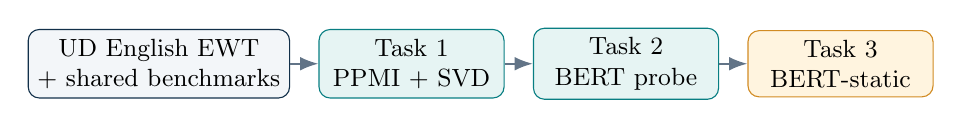
\begin{tikzpicture}[node distance=0.36cm,>=Latex,every node/.style={font=\small,align=center}]
\node[draw=Navy,fill=Pale,rounded corners,minimum width=2.55cm,minimum height=0.78cm] (data) {UD English EWT\\+ shared benchmarks};
\node[draw=Teal,fill=TealLight,rounded corners,minimum width=2.35cm,minimum height=0.78cm,right=of data] (t1) {Task 1\\PPMI + SVD};
\node[draw=Teal,fill=TealLight,rounded corners,minimum width=2.35cm,minimum height=0.78cm,right=of t1] (t2) {Task 2\\BERT probe};
\node[draw=Gold,fill=GoldLight,rounded corners,minimum width=2.35cm,minimum height=0.78cm,right=of t2] (t3) {Task 3\\BERT-static};
\draw[->,thick,Muted] (data)--(t1); \draw[->,thick,Muted] (t1)--(t2); \draw[->,thick,Muted] (t2)--(t3);
\end{tikzpicture}
\tinycaption{Both codebases separate the three tasks, while sharing the same data and benchmark definitions.}
\end{frame}

% ------------------------------------------------------------ 5 cross-check
\begin{frame}{Cross-check: same settings $\Rightarrow$ same numbers}
\begin{columns}[T,onlytextwidth]
\column{0.64\textwidth}
\scriptsize
\begin{tabularx}{\linewidth}{@{}Xcc@{}}
\toprule
Quantity & \A{} re-scored in \B's setting & \B{} reported \\
\midrule
Types with count $\geq 2$ & 8,865 & 8,865 \\
Analogy questions, all words count $\geq 2$ & 3,406 & 3,406 \\
T3 WS-353 $\rho$ on the same 203 pairs & \hl{\XTThreeSub} & \hl{\BTSameWS} \\
T3 WS-353 $\rho$, all 353, missing $=0$ & \hl{\XTThreeAllZero} & \hl{0.288} \\
T3 WS-353 $\rho$, 248 covered pairs & \TThreeWSCov & \BTAllWS \\
T3 analogy, covered / all questions & \TThreeANCov\% / \TThreeANFull\% & \BTAllAN\% / 19.8\% \\
\midrule
T1 WS-353 $\rho$ on the 203 pairs & \XTOneSub & \BWSCov \\
\bottomrule
\end{tabularx}
\column{0.33\textwidth}
\begin{exampleblock}{What the cross-check establishes}
\begin{itemize}\tightitem
\item The Task 3 pipelines are equivalent: matched figures agree to three decimals.
\item Restricting to 8,865 types changes the analogy candidate set and pair coverage.
\item Task 1 differs because \B{} removes singleton words before SVD.
\end{itemize}
\end{exampleblock}
\end{columns}
\vspace{0.25em}
\begin{beamercolorbox}[rounded=true,sep=0.8ex,wd=\linewidth]{block body}
\textbf{Why this control is important:} a fair implementation comparison must hold vocabulary, scored item set, missing-value policy, and analogy candidates fixed. Otherwise a score change can come from evaluation coverage rather than model quality.
\end{beamercolorbox}
\vspace{0.18em}
\begin{beamercolorbox}[rounded=true,sep=0.65ex,wd=\linewidth]{block body example}
\centering\small\textbf{Matched evaluation set:} 8,865 word types $\;\vert\;$ 203 common WordSim pairs $\;\vert\;$ 3,406 common analogy questions.
\end{beamercolorbox}
\end{frame}

% ------------------------------------------------------------ 6 T1
\begin{frame}{Task 1: both find weak, data-limited vectors}
\begin{columns}[T,onlytextwidth]
\column{0.59\textwidth}
\footnotesize
\begin{tabularx}{\linewidth}{@{}Xcc@{}}
\toprule
Task 1: PPMI--SVD & \A & \B \\
\midrule
WS-353 $\rho$, covered pairs & \TOneWSCov{} (248) & \BWSCov{} (203) \\
WS-353 $\rho$, all 353 & \TOneWSFull{} (median) & \BWSAllZero{} (zero) \\
Analogy accuracy, covered & \TOneANCov\% & \BANCov\% \\
MST UUAS, 20 sentences & \TOneMST\% & \BMSTTwenty\% \\
\quad random / linear-chain baseline & \RandomMST{} / \ChainMST & \BRandTwenty{} / \BChainTwenty \\
MST UUAS, larger set & \TOnePool\% (660) & \BMSTFull\% (1,926) \\
\bottomrule
\end{tabularx}
\vspace{0.22em}
\begin{exampleblock}{What the baseline is learning}
\small Co-occurrence within a symmetric $\pm 5$ window captures topical partners. The neighbour examples confirm this: \emph{monday} $\to$ Friday / July / Tuesday; \emph{good} $\to$ nice / food / great. The small corpus still gives sparse counts and weak similarity estimates.
\end{exampleblock}
\column{0.38\textwidth}
\begin{block}{Agreement across runs}
\begin{itemize}\tightitem
\item WordSim correlation is near zero when all 353 pairs are included.
\item Google analogy accuracy remains below 1\% on covered questions.
\item MST scores exceed random trees but remain far below a linear chain.
\end{itemize}
\end{block}
\begin{alertblock}{Why covered $\rho$ differs}
\small \B's 203 covered pairs exclude rare words. On this same subset, \A's Task 1 vectors score \XTOneSub{}; this is a coverage effect, not evidence of a stronger model.
\end{alertblock}
\end{columns}
\vspace{0.25em}
\begin{beamercolorbox}[rounded=true,sep=0.75ex,wd=\linewidth]{block body}
\textbf{Pipeline:} EWT training text $\rightarrow$ word--word co-occurrence matrix $\rightarrow$ PPMI weighting $\rightarrow$ truncated SVD (100 dimensions) $\rightarrow$ cosine similarity / vector-offset analogy / sentence MST.
\end{beamercolorbox}
\end{frame}

% ------------------------------------------------------------ 7 T2
\begin{frame}{Task 2: same best layer, different absolute UUAS}
\begin{columns}[T,onlytextwidth]
\column{0.66\textwidth}
\centering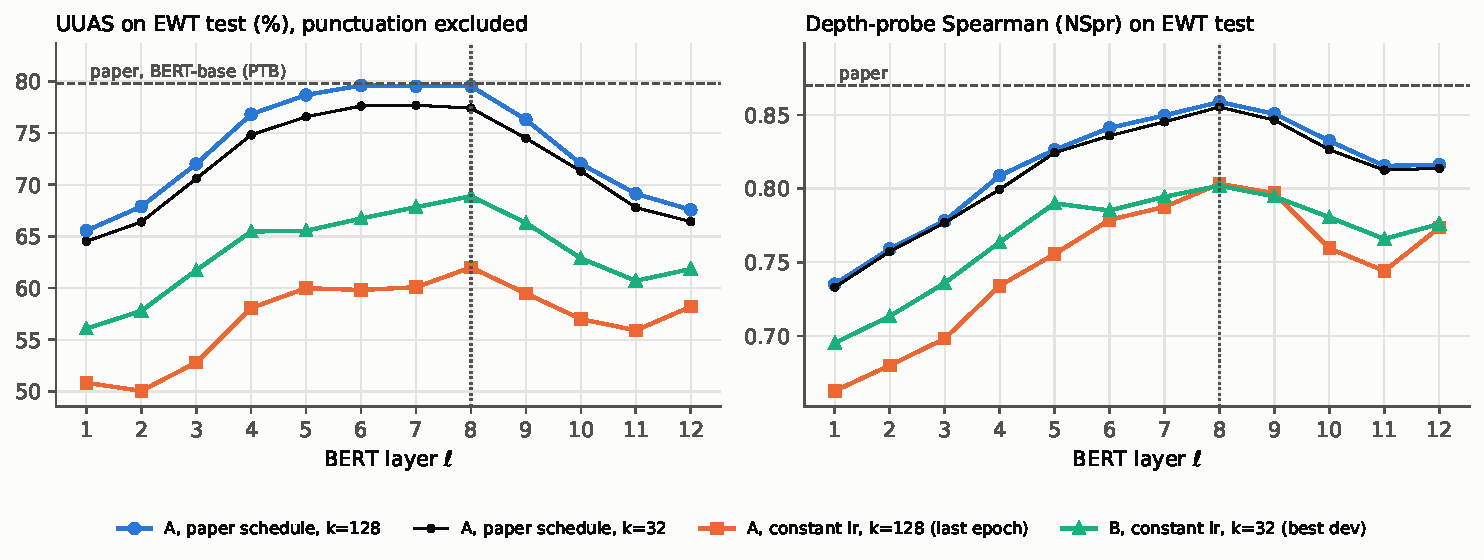
\includegraphics[width=\linewidth,height=4.55cm,keepaspectratio]{fig_layers_cmp.pdf}
\tinycaption{Layer-wise test performance. The mid-layer peak appears in both runs; the absolute level depends strongly on the optimization schedule.}
\column{0.32\textwidth}
\metric{\lstar = 8}{best syntax layer in both implementations}
\vspace{0.2em}
\footnotesize
\begin{tabular}{@{}lcc@{}}
\toprule
 & UUAS & NSpr \\
\midrule
Paper (PTB) & 79.8 & 0.87 \\
\A, lr decay & \TtwoTestUuas & \TtwoTestNspr \\
\B, constant lr & \BUUASnp & \BNSpr \\
\A, constant lr & \ALitUUASonetwoeight & \LitNspr \\
\bottomrule
\end{tabular}
\vspace{0.15em}
\begin{exampleblock}{Interpretation}
\scriptsize Both independently identify layer 8. With the paper-style schedule, \A{} reaches 79.5\% UUAS, close to the 79.8\% paper reference.
\end{exampleblock}
\end{columns}
\vspace{0.15em}
\begin{beamercolorbox}[rounded=true,sep=0.65ex,wd=\linewidth]{block body}
\scriptsize\textbf{Probe setup:} frozen BERT layers 1--12; linear distance and depth projections; ranks $k\in\{32,64,128\}$; Adam; MST decoding of predicted pairwise distances; choose $\lstar$ on the dev split and report UUAS / depth-probe Spearman on test.
\end{beamercolorbox}
\end{frame}

% ------------------------------------------------------------ 8 schedule + relation recall
\begin{frame}{Why the UUAS differs: learning-rate schedule and relation difficulty}
\begin{columns}[T,onlytextwidth]
\column{0.49\textwidth}
\begin{block}{Evidence from the two runs}
\small
\begin{itemize}\tightitem
\item \A's control with constant lr drops to \ALitUUASonetwoeight\% (last epoch); \B{} reports \BUUASnp\% using its best-dev epoch.
\item \B's best $k=128$ checkpoint is mostly epoch 1. \A's constant-lr dev minimum is also at epoch \LitMinEpoch, then it oscillates for 29 epochs.
\item Training loss remains high (0.62 vs. 0.42 with decay): this is non-convergence, not over-fitting.
\item Rank preference also flips: constant lr favours $k=32$; decay favours $k=128$ (77.4 / 79.2 / 79.5\%), as in the paper.
\end{itemize}
\end{block}
\begin{alertblock}{Mechanism}
\small With a constant step size, Adam keeps moving around the minimum. The paper's $\times 0.1$ decay after a dev plateau reduces the step size and lets the probe settle.
\end{alertblock}
\column{0.49\textwidth}
\centering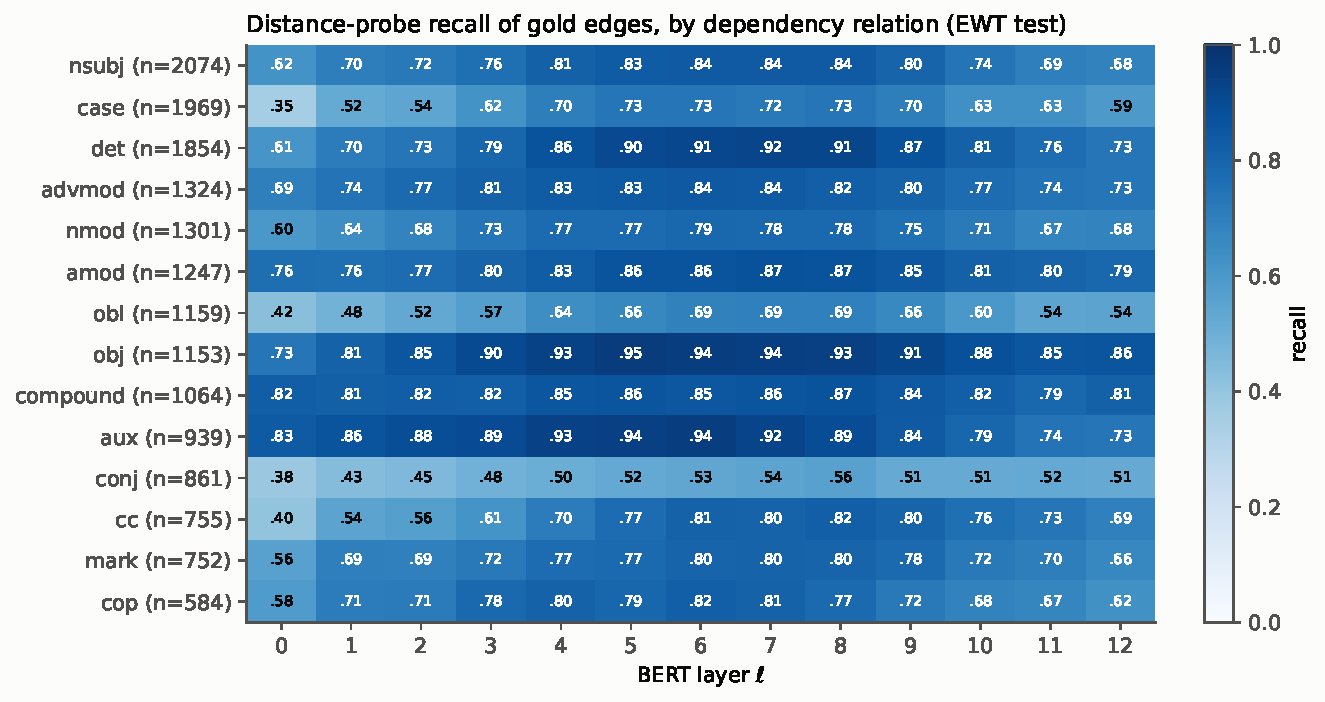
\includegraphics[width=0.95\linewidth,height=4.25cm,keepaspectratio]{relation_recall_heatmap.pdf}
\tinycaption{\A's layer-wise recall of gold dependency edges by relation on EWT test.}
\begin{beamercolorbox}[rounded=true,sep=0.65ex,wd=\linewidth]{block body example}
\scriptsize\textbf{What is easier / harder?} Short local relations such as object (0.93), determiner (0.91), and auxiliary (0.89) are recovered well. Coordination (conj, 0.56) and oblique attachment (obl, 0.69) are harder.
\end{beamercolorbox}
\end{columns}
\end{frame}

% ------------------------------------------------------------ 9 qualitative Task 2
\begin{frame}{Task 2: what the probe gets right -- and where it fails}
\begin{columns}[T,onlytextwidth]
\column{0.49\textwidth}
\begin{block}{Typical test sentence: UUAS = \QTypicalUUAS}
\centering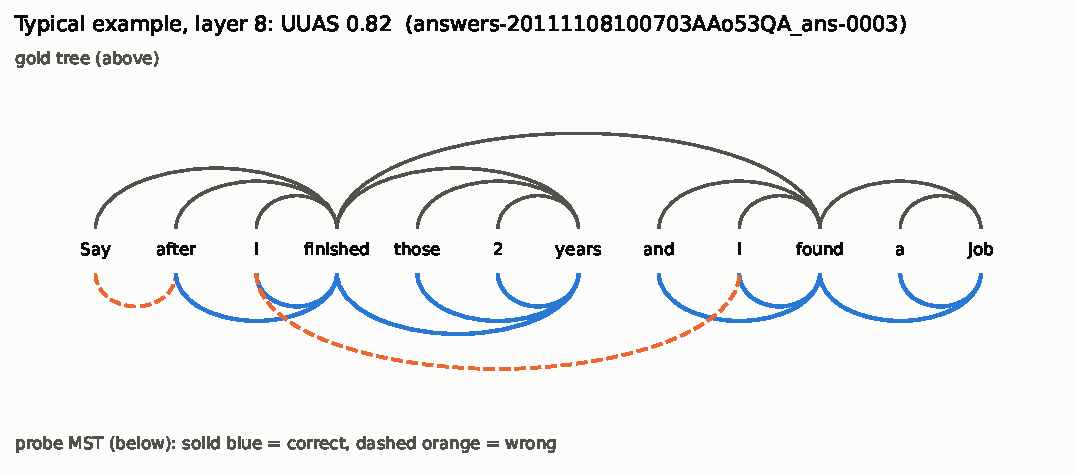
\includegraphics[width=\linewidth,height=2.65cm,keepaspectratio]{example_typical.pdf}
\scriptsize\textbf{Reading:} short web sentence; most local arcs are recovered, but discourse and coordination links are fragile.
\end{block}
\scriptsize
\textbf{Observed errors:} misses the discourse attachment Say--finished and the conjunct link finished--found; adds Say--after and I--I.
\column{0.49\textwidth}
\begin{alertblock}{Poor test sentence: UUAS = \QPoorUUAS}
\centering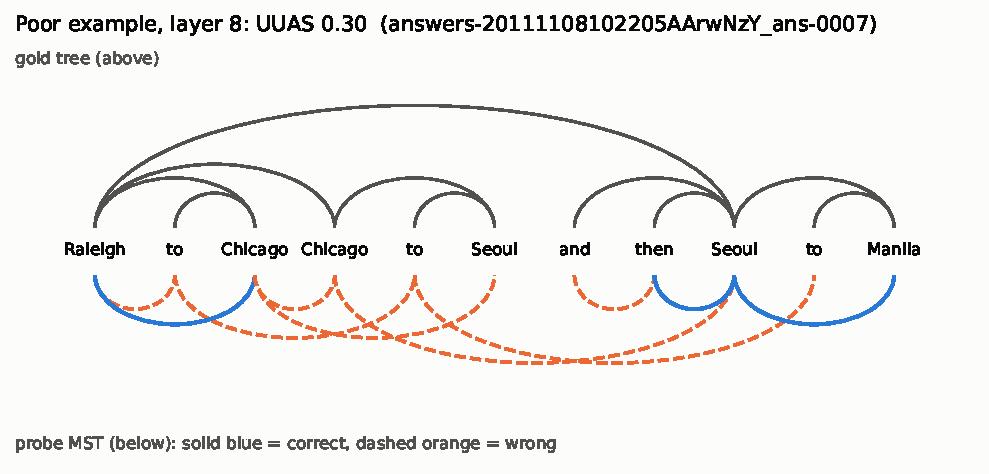
\includegraphics[width=\linewidth,height=2.65cm,keepaspectratio]{example_poor.pdf}
\scriptsize\textbf{Reading:} repeated city names and prepositions cause lexical-identity links to compete with syntactic relations.
\end{alertblock}
\scriptsize
\textbf{Observed errors:} a verbless itinerary with repeated word forms; the probe creates spurious links such as to--to and Chicago--Chicago.
\end{columns}
\vspace{0.35em}
\begin{exampleblock}{What these examples reveal}
\small Layer-8 BERT representations contain useful syntactic geometry, but similar lexical forms can still dominate pairwise distances. The probe is strong in aggregate, not uniformly correct sentence by sentence.
\end{exampleblock}
\end{frame}

% ------------------------------------------------------------ 10 T3 meaning
\begin{frame}{Task 3, meaning: both find a large gain}
\begin{columns}[T,onlytextwidth]
\column{0.51\textwidth}
\footnotesize
\begin{tabular}{@{}llcc@{}}
\toprule
 & System & WS $\rho$ & Analogy \\
 & & (203 pairs) & (covered) \\
\midrule
\A & T1 PPMI--SVD & 0.171 & 0.51\% \\
\B & T1 PPMI--SVD & 0.189 & 0.85\% \\
\midrule
\A & T3 BERT-static, L8 & \hl{\XTThreeSub} & \hl{67.7\%} \\
\B & T3 BERT-static, L8 & \hl{\BTSameWS} & \hl{77.1\%} \\
\midrule
\A & T3 + all-but-the-top & \hl{\XTThreeASub} & 71.0\% \\
\B & T3 mean-centred & \hl{0.706} & 78.3\% \\
\bottomrule
\end{tabular}
\vspace{0.2em}
\begin{exampleblock}{Statistical evidence (A)}
\scriptsize $\Delta\rho=\PtWSDiff$ with 95\% CI \PtWSCI. T3 solves \PtANOnlyA{} analogy questions missed by T1; the reverse count is \PtANOnlyB.
\end{exampleblock}
\column{0.47\textwidth}
\begin{block}{Why the gain is large}
\small
\begin{itemize}\tightitem
\item WordSim $\rho$ rises from about 0.18 to 0.65 on the matched 203 pairs.
\item Covered analogy accuracy moves from below 1\% to 68--77\%.
\item Removing the dominant shared direction improves T3 in both implementations.
\item \B's analogy candidate set is restricted to 8,865 words, raising its covered accuracy.
\end{itemize}
\end{block}
\begin{alertblock}{Important comparison caveat}
\small This is not a data-matched pre-training comparison: BERT already learned from approximately 3.3B words; EWT supplies the contexts used for pooling.
\end{alertblock}
\end{columns}
\vspace{0.2em}
\begin{beamercolorbox}[rounded=true,sep=0.65ex,wd=\linewidth]{block body}
\scriptsize\textbf{Layer distinction:} the best syntax layer is 8, but semantic static-vector quality peaks earlier; the full layer sweep is shown next.
\end{beamercolorbox}
\end{frame}

% ------------------------------------------------------------ 11 layer sweep
\begin{frame}{Task 3, layer sweep: the best layer depends on the target}
\begin{columns}[T,onlytextwidth]
\column{0.66\textwidth}
\centering
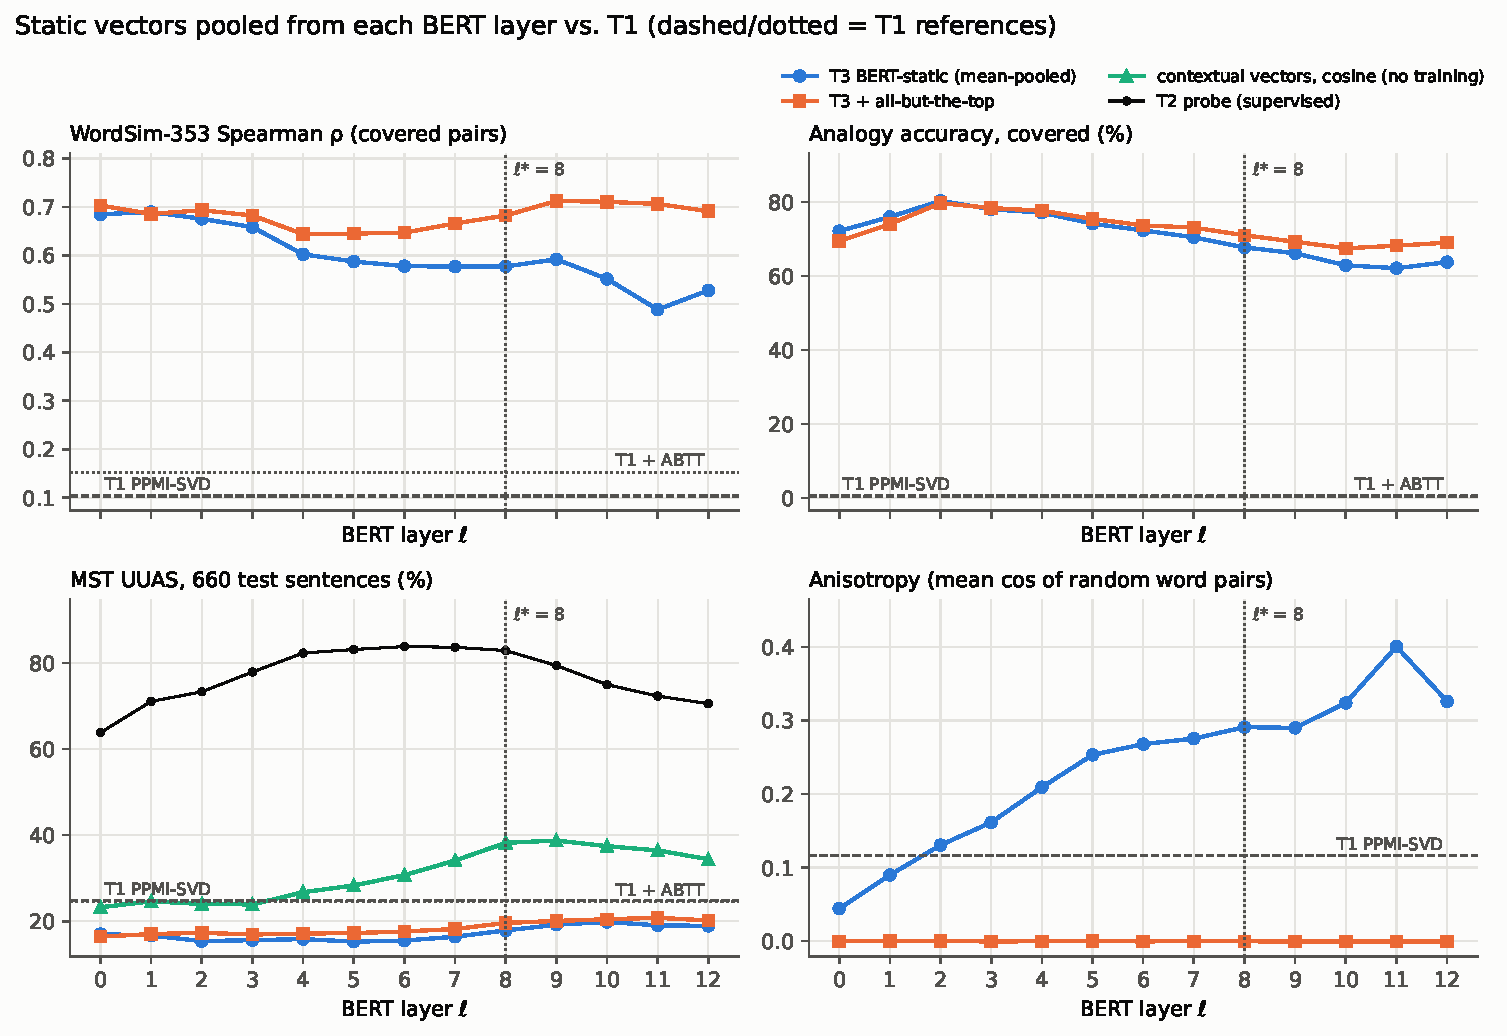
\includegraphics[width=\linewidth,height=5.35cm,keepaspectratio]{layer_sweep.pdf}
\column{0.32\textwidth}
\begin{exampleblock}{Word meaning}
\small WordSim-353 peaks at layer 1 (A: 0.690; B: 0.723 on the matched pair set).
\end{exampleblock}
\begin{exampleblock}{Analogical structure}
\small Google analogy accuracy peaks at layer 2 (A: 80.3\%; B: 86.2\%).
\end{exampleblock}
\begin{alertblock}{Syntax / tree check}
\small Probe UUAS peaks at layer 8; static MST is best around layer 10 but remains near chance.
\end{alertblock}
\end{columns}
\end{frame}

% ------------------------------------------------------------ 12 T3 structural
\begin{frame}{Task 3, trees: both find no improvement}
\begin{columns}[T,onlytextwidth]
\column{0.55\textwidth}
\footnotesize
\begin{tabular}{@{}lcccc@{}}
\toprule
 & \multicolumn{2}{c}{20 sentences} & \multicolumn{2}{c}{larger set} \\
UUAS (\%) & \A & \B & \A{} (660) & \B{} (1,926) \\
\midrule
Random tree & \RandomMST & \BRandTwenty & \RandomPool & \BRandFull \\
Linear chain & \ChainMST & \BChainTwenty & \ChainPool & \BChainFull \\
\midrule
T1 PPMI--SVD & \TOneMST & \BMSTTwenty & \TOnePool & \BMSTFull \\
T3 BERT-static & \warn{\TThreeMST} & \warn{\BTSameMST} & \warn{\TThreePool} & \warn{\BTSameFull} \\
T3 + anisotropy fix & \TThreeAMST & \BTCenMST & \TThreeAPool & \BTCenFull \\
\midrule
T2 probe (A) & \TTwoRefMST & -- & \TTwoRefPool & -- \\
\bottomrule
\end{tabular}
\vspace{0.25em}
\begin{alertblock}{Result across both implementations}
\small T3 is below T1 in both samples and remains close to the random-tree baseline. Better semantic similarity does not translate into better sentence-tree recovery.
\end{alertblock}
\begin{exampleblock}{Significance (A)}
\scriptsize 20-sentence change: $\Delta=\PtMSTDiff$ pt, not significant. 660-sentence change: $\Delta=\PtPoolDiff$ pt, CI \PtPoolCI.
\end{exampleblock}
\column{0.43\textwidth}
\centering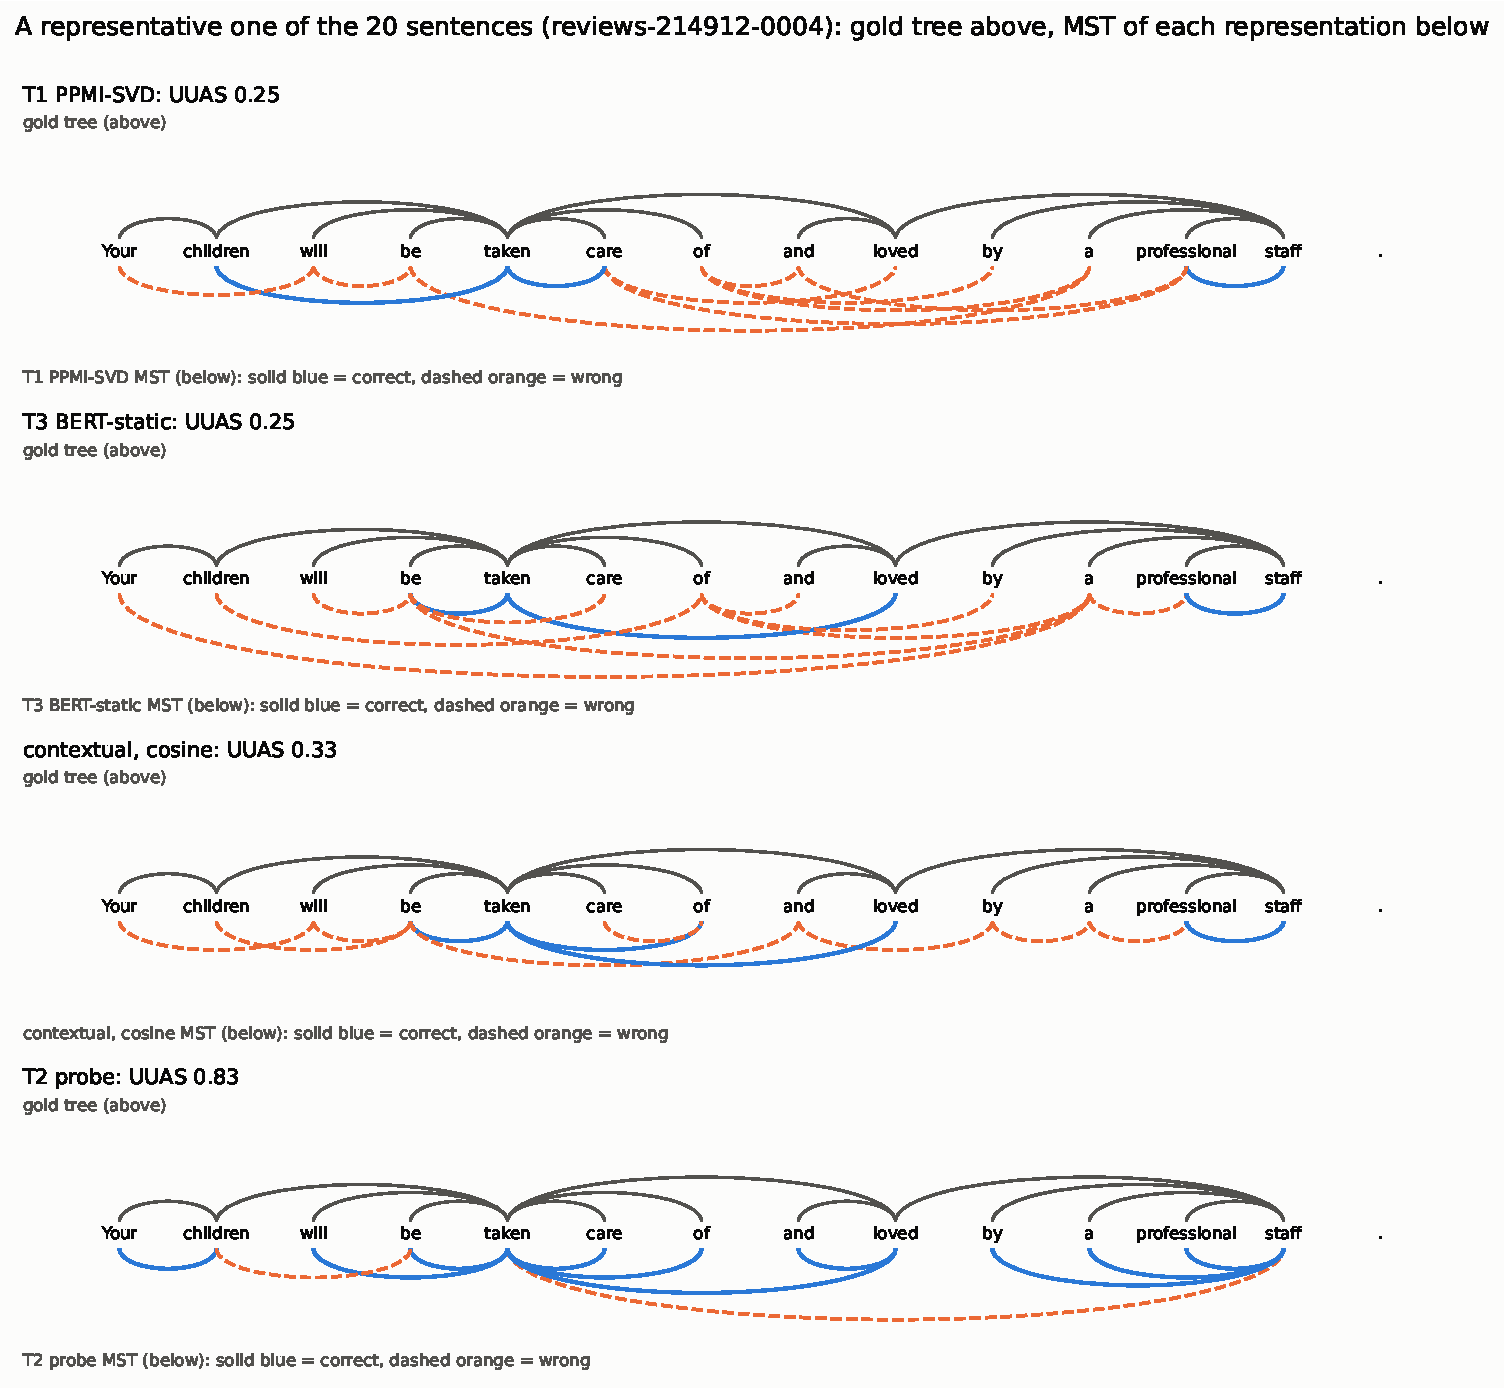
\includegraphics[width=\linewidth,height=4.9cm,keepaspectratio]{mst_example.pdf}
\tinycaption{Representative EWT sentence: T1, T3, contextual cosine, and the learned probe yield very different trees.}
\end{columns}
\end{frame}

% ------------------------------------------------------------ 12 why
\begin{frame}{Why meaning and syntax disagree: from word types to token relations}
\begin{columns}[T,onlytextwidth]
\column{0.48\textwidth}
\begin{block}{Explanation from implementation B}
\small
\begin{itemize}\tightitem
\item Pooling averages away context-specific information.
\item The structural probe learns a projection; the MST check uses raw cosine distances.
\item BERT-static neighbours act like semantic substitutes, while syntax depends on relations between words in context.
\item OOV words can inject arbitrary distances into B's MST sample (7.4\% of tokens).
\end{itemize}
\end{block}
\begin{alertblock}{A's quantitative diagnostics}
\scriptsize On T3, 0.74 of nearest neighbours share the same POS (T1: 0.33; random: 0.22). T1 neighbours co-occur 0.56 of the time (T3: 0.16; random: 0.07).\\[2pt]
\textbf{Interpretation:} static neighbours are semantic substitutes; dependency edges connect contextual partners.
\end{alertblock}
\column{0.50\textwidth}
\begin{center}
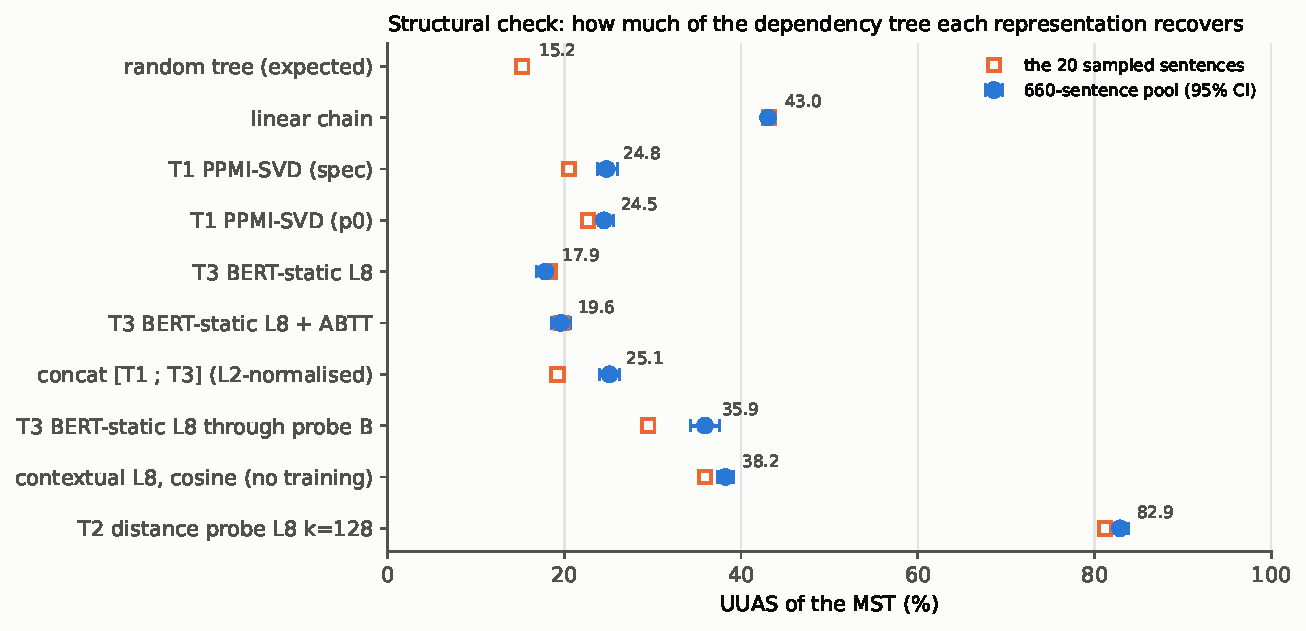
\includegraphics[width=0.99\linewidth,height=3.95cm,keepaspectratio]{ladder.pdf}
\tinycaption{Same 660-sentence sample: each step restores a more syntax-aware signal.}
\end{center}
\begin{exampleblock}{Does geometric closeness predict a gold edge?}
\scriptsize Edge AUC: T3 static \warn{\AucTThree}; T1 static \AucTOne; contextual cosine \AucCtx; learned probe \hl{\AucProbe}. The trained projection is much more syntax-aligned than raw static-vector geometry.
\end{exampleblock}
\end{columns}
\end{frame}

% ------------------------------------------------------------ 13 robust vs sensitive
\begin{frame}{What survives a change of implementation?}
\begin{columns}[T,onlytextwidth]
\column{0.49\textwidth}
\begin{exampleblock}{Robust: both implementations agree}
\begin{itemize}\tightitem
\item $\lstar=8$: syntax is strongest in the middle layers, then declines toward layer 12.
\item T3 $\gg$ T1 on WordSim-353 and analogies.
\item T3 $<$ T1 on the MST check; tree recovery remains close to random.
\item Static semantics peaks at layers 1--2, not at syntax layer 8.
\item Centering / all-but-the-top improves T3 semantic quality.
\item T3 numbers match exactly once vocabulary and evaluation settings are aligned.
\end{itemize}
\end{exampleblock}
\column{0.49\textwidth}
\begin{alertblock}{Implementation-sensitive: raw values move}
\begin{itemize}\tightitem
\item Probe UUAS ranges from 62\% to about 80\% with learning-rate schedule / checkpoint choice.
\item Best probe rank changes: 32 vs. 128.
\item T1 WordSim $\rho$ changes from 0.10 to 0.17--0.19 with pair subset and vocabulary cutoff.
\item MST levels differ by up to 8 points with sentence sample and punctuation.
\item ``All 353'' $\rho$ depends on the OOV imputation rule.
\end{itemize}
\end{alertblock}
\end{columns}
\vspace{0.03em}
\begin{beamercolorbox}[rounded=true,sep=0.4ex,wd=\linewidth]{block body}
\textbf{Reproducibility lesson:} report vocabulary thresholds, benchmark coverage, OOV handling, punctuation policy, probe rank, checkpoint rule, and learning-rate schedule. These choices can move the reported number more than the effect being investigated.
\end{beamercolorbox}
\end{frame}

% ------------------------------------------------------------ 14 conclusions
\begin{frame}{Conclusions}
\begin{columns}[T,onlytextwidth]
\column{0.32\textwidth}\metric{T1}{PPMI--SVD baseline}\vspace{0.12em}\centering\Large\bfseries\color{Navy}$\rho\approx0.1$--$0.19$\\[-1pt]{\scriptsize Analogies below 1\%}
\column{0.32\textwidth}\metric{T2}{Structural probe}\vspace{0.12em}\centering\Large\bfseries\color{Navy}79.5\%\\[-1pt]{\scriptsize UUAS with paper-style schedule}
\column{0.32\textwidth}\metric{T3}{BERT-static, layer 8}\vspace{0.12em}\centering\Large\bfseries\color{Navy}$\rho=0.648$\\[-1pt]{\scriptsize 67.7--77.1\% analogy accuracy}
\end{columns}
\vspace{0.25em}
\begin{enumerate}\tightitem
\item \textbf{Task 1:} classical vectors from only 204k training tokens are weak and data-limited in both implementations.
\item \textbf{Task 2:} BERT encodes dependency structure in a low-rank subspace of its middle layers; both identify $\lstar=8$.
\item \textbf{Task 3:} pooling layer-8 contextual vectors greatly improves word meaning, but weakens dependency-tree recovery compared with Task 1.
\item The disagreement is not a contradiction: type-level semantic similarity and token-level syntactic relations are different targets.
\item Two independent implementations make the conclusions more robust and reveal which experimental choices are sensitive.
\end{enumerate}
\vspace{0.3em}
\begin{beamercolorbox}[rounded=true,sep=1.05ex,wd=\linewidth]{block body example}
\centering\large\bfseries\color{Navy}A good static meaning vector is not automatically a good syntactic representation.
\end{beamercolorbox}
\end{frame}

% ------------------------------------------------------------ 15 references
\begin{frame}{References}
\footnotesize
\begin{columns}[T,onlytextwidth]
\column{0.49\textwidth}
\begin{itemize}\tightitem
\item J. Hewitt and C. D. Manning (2019). \emph{A structural probe for finding syntax in word representations}. NAACL.
\item O. Levy and Y. Goldberg (2014). \emph{Neural word embedding as implicit matrix factorization}. NeurIPS.
\item R. Bommasani, K. Davis, and C. Cardie (2020). \emph{Interpreting pretrained contextualized representations via reductions to static embeddings}. ACL.
\item J. Devlin et al. (2019). \emph{BERT: Pre-training of deep bidirectional transformers for language understanding}. NAACL.
\end{itemize}
\column{0.49\textwidth}
\begin{itemize}\tightitem
\item J. Mu and P. Viswanath (2018). \emph{All-but-the-top: simple and effective postprocessing for word representations}. ICLR.
\item K. Ethayarajh (2019). \emph{How contextual are contextualized word representations?} EMNLP.
\item M. Sahlgren (2006). \emph{The Word-Space Model}. PhD thesis, Stockholm University.
\item M.-C. de Marneffe et al. (2021). \emph{Universal Dependencies}. Computational Linguistics, 47(2).
\end{itemize}
\end{columns}
\vspace{0.22em}
\begin{exampleblock}{Project materials}
\small Combined report: \texttt{Combined/report\_combined.pdf}; individual implementation reports and experiment outputs in each author's folder; code repository: \url{https://github.com/trishitasaha/NLP_Assignment2}.
\end{exampleblock}
\vspace{0.3em}
\begin{beamercolorbox}[rounded=true,sep=0.8ex,wd=\linewidth]{block body}
\scriptsize Benchmark results and implementation comparisons in this presentation are taken from the supplied combined report. All A/B differences are interpreted with the report's vocabulary, OOV, sample-size, and punctuation caveats.
\end{beamercolorbox}
\end{frame}

\end{document}
